\chapter{Introduzione}
\lettrine[lines=2]{S}{econdo} le indagini effettuate dall'Associazione Italiana per la Sicurezza Informatica (CLUSIT) e racchiuse nel loro rapporto 2025 sulla Cybersecurity in Italia e nel mondo, negli ultimi 5 anni il numero degli incidenti globali rilevati è cresciuto esponenzialmente passando in media mensile dai 156 del 2020 ai 295 del 2024 (+27\% dal 2023 al 2024). Un 80\% di questi incidenti sono ritenuti "gravi" o "critici".\cite{clusit}\\[1em]
Inoltre, con l'ascesa dell'AI nel panorama della cyber sicurezza, molte sono le aziende del settore ad aver iniziato ad utilizzare i vantaggi e i tool resi disponibili dalla nuova tecnologia ormai in continua crescita nel mercato globale. In Italia in particolare si stima una dimensione del mercato di 4.12 miliardi USD per il 2025 con la previsione di toccare i 7.59 miliardi entro il 2030.\cite{mordor} \\[1em]
L'intelligenza artificiale svolge un ruolo fondamentale nell'identificazione di minacce o nell'automazione di compiti quali analisi dei log o scanning di vulnerabilità ma, il rovescio della medaglia è che l'intelligenza artificiale viene sfruttata anche dalle organizzazioni di Advance Threat Persistance (APT) per creare dei tipi di attacco che sfruttano, in special modo, il Natural Language Processing\footnotemark{} ed implementare minacce sempre più efficaci e ostili, anche verso il più vigilante degli utenti.

\begin{figure}[htbp]
    \centering
    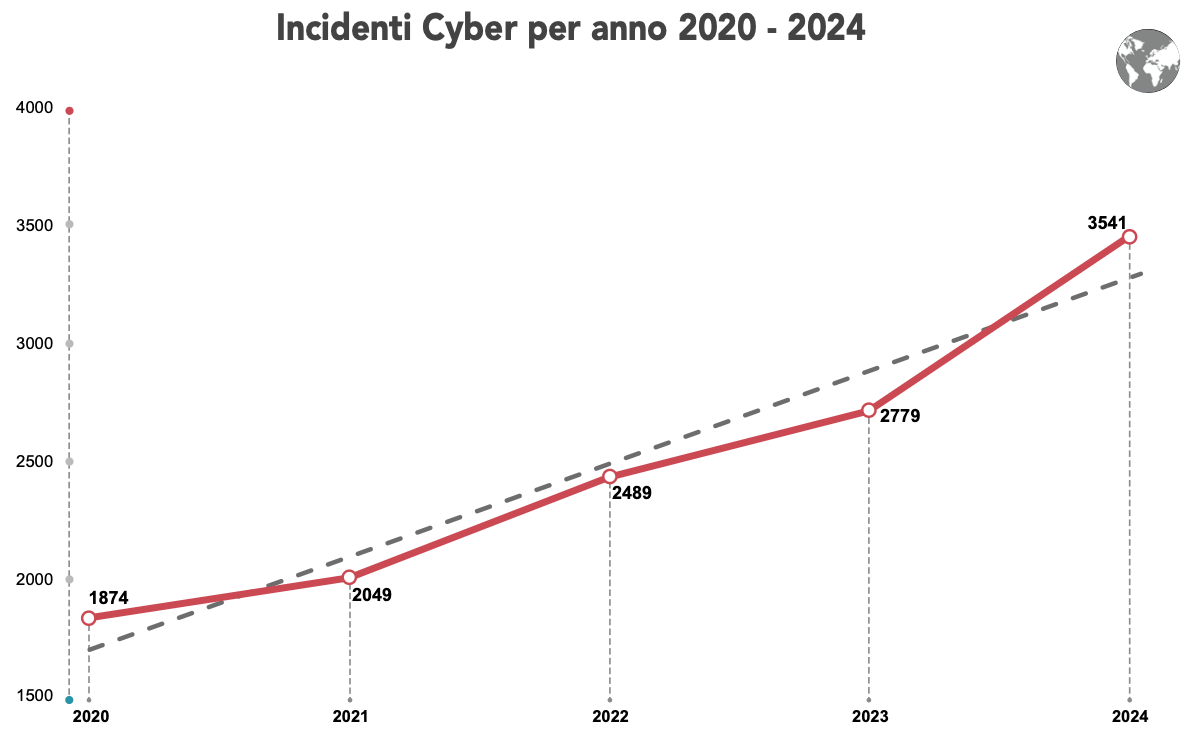
\includegraphics[width=0.7\linewidth]{images/Clusit_graph.png}
    \caption{Andamento incidenti anno 2020 - 2024 \cite[]{clusit}} 
\end{figure}

\footnotetext{NLP - Sottocampo dell'Intelligenza Artificiale, utilizza il machine learning per consentire al computer di poter comprendere e comunicare con il linguaggio umano.}

\begin{figure}
    \centering
    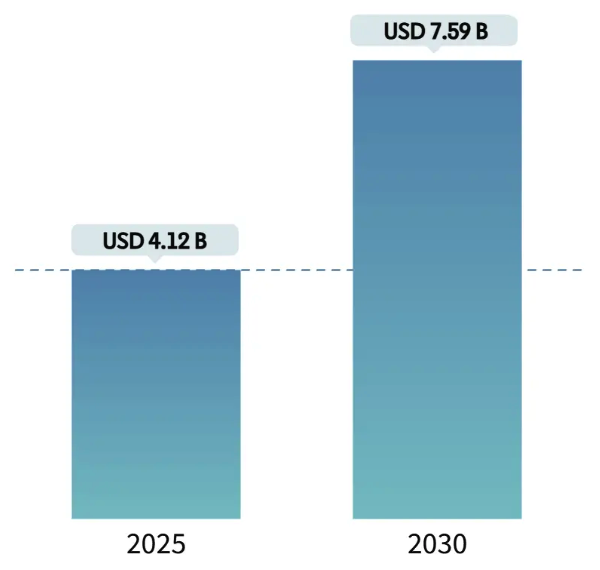
\includegraphics[width=0.5\linewidth]{images/Mordor_stat.png}
    \caption{Dimensione del mercato AI in Italia 2025 e 2030 \cite{mordor}}
\end{figure}

\section{Concetti fondamentali}
Fin dall'alba dei conflitti militari, è stato di vitale importanza l'usufruire di simulazioni e wargames in modo da addestrare e preparare gli ufficiali ad imminenti minacce e rafforzare le proprie difese.\\
I termini "Red Team" e "Blue Team" fanno la loro prima comparsa ufficiale durante gli anni 60', il Dipartimento di Difesa degli Stati Uniti (DoD) usò i suddetti termini per riferirsi ad astrazioni strutturate usate per testare strategie di alto livello.

    \subsection{Red Team\label{red}}
    Un Red Team è un gruppo di esperti in sicurezza informatica all'interno di un'organizzazione, con lo scopo di violare le sue stesse misure di difesa e seguendo una determinata policy. In questo modo si identificano le vulnerabilità prima che queste vengano sfruttate da entità malevole.\\
    Lo scopo principale della squadra consiste nel riuscire ad emulare, nel modo più realistico possibile, un attacco all'organizzazione da parte di un attore maligno. L'organizzazione, da parte sua, grazie al lavoro del team, sarà in grado di vedere all'opera la struttura delle proprie difese, annotare come esse rispondono ad un'improvvisa aggressione ed eventualmente migliorarle o colmare delle lacune riscontrate durante i test tramite delle patch di sicurezza.\\[1.5em]
    {\bfseries\Large Tattiche e Strategie}\\[1.5em]
    La squadra si avvale di diverse tattiche, tecniche e procedure (TTPs) durante lo svolgimento dell'operazione. È compito dell'enterprise stabilire i limiti e le regole di ingaggio standard da utilizzare durante il lavoro. Di seguito, una lista delle fasi più comuni durante gli attacchi:
    \begin{itemize}
        \item \textbf{Social Engineering:} Mira principalmente i dipendenti di un'azienda, consiste nell'arte di manipolare le persone toccando leve psicologiche e comportamentali, in modo da ottenere informazioni sensibili riguardo l'environment target. Si differenzia dalle altre tecniche perchè agisce sulle debolezze del singolo individuo: il cybercriminale inizia col raccogliere dati personali, studiare le abitudini, costruire un rapporto di fiducia apparente e, infine, colpire un'area emotiva sensibile della vittima bersaglio (paura, curiosità, emergenza, ecc...) in modo da costringerla a rivelare delle informazioni vitali per il proseguimento dell'infiltrazione.
        \item \textbf{Network Scanning:} È considerato il primo passo verso l'infiltrazione perché permette di ricostruire il sistema di rete e sfruttare le vulnerabilità riscontrate; esso consiste nel ricercare tutti i servizi TCP e UDP disponibili negli host della rete bersaglio con annessi dati riguardanti il sistema operativo, server database presenti e simili.\\
        Vi sono due principali strumenti utilizzati per la fase di scanning:
        \begin{enumerate}
            \item \textbf{ARP:} Un protocollo di rete situato al livello di collegamento del modello di rete ISO/OSI, permette di mappare degli indirizzi IP della rete LAN agli indirizzi MAC fisici dei dispositivi collegati.\\
            È possibile sfruttare delle richieste ARP broadcast in modo da interagire con chiunque abbia un indirizzo nella rete; dopo aver inviato un segnale ad un determinato host, si incrementa di uno l'indirizzo IP di destinazione fino a scandirli tutti. Alla fine, gli host con un IP corrispondente risponderanno alla richiesta. Il principale svantaggio di questo metodo consiste nel doversi limitare alla sottorete in cui viene effettuata la scannerizzazione: ad esempio, se la squadra si trova in una rete 10.10.10.0/24\footnotemark mentre il target è in 172.172.172.0/24, dalla prima famiglia di indirizzi non è possibile inviare dei segnali ARP alla seconda.\\
            In compenso, è molto veloce, efficiente e nella maggior parte di casi non genera nessun segnale d'allarme.\\[1.5em]
            \begin{figure}[H]
                \vspace{-1.5em}
                \centering
                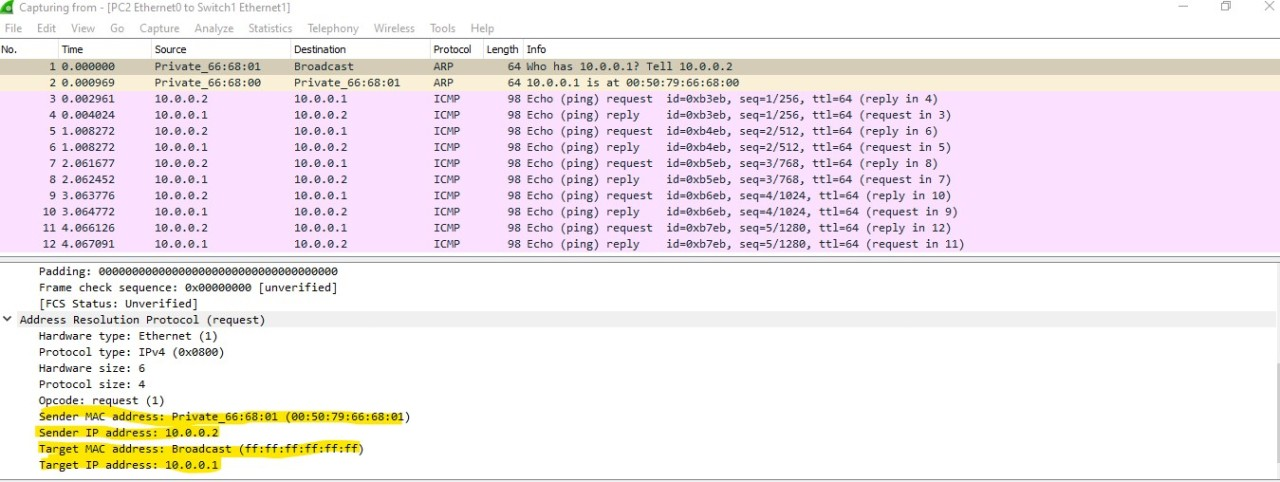
\includegraphics[width=\linewidth]{images/ARP.jpeg}
                \caption{ Esempio di ARP request in Wireshark }
            \end{figure}
\footnotetext{Notazione CIDR - Rappresenta la famiglia di indirizzi disponibili nella rete composta dai primi 24 bit. Si estende da 10.10.10.1 fino a 10.10.10.254.}
            \item \textbf{NMAP:} Letteralmente \textit{"Network Mapper"}, è il tool più popolare utilizzato se stiamo parlando di scanning della rete ed identificazione delle debolezze; difatti è il comando cardine utilizzato nel mio lavoro di progettazione della VM vulnerabile nonché un alleato prezioso per i Red Teams.\\
            Rilasciato per la prima volta nel 1997 da Gordon Lyon, riesce ad identificare hosts e servizi all'interno di una rete tramite l'invio di pacchetti (per esempio, TCP o ICMP) e l'analisi delle risposte da parte dei sistemi. Numerose sono le sue funzionalità, che possono essere sfruttate al meglio aggiungendo ad un semplice comando degli scripts per conoscere le difese della vittima quali firewall, sistema operativo, porte di servizi aperte, ecc...\cite{nmap}\\
            \begin{figure}[H]
                \centering
                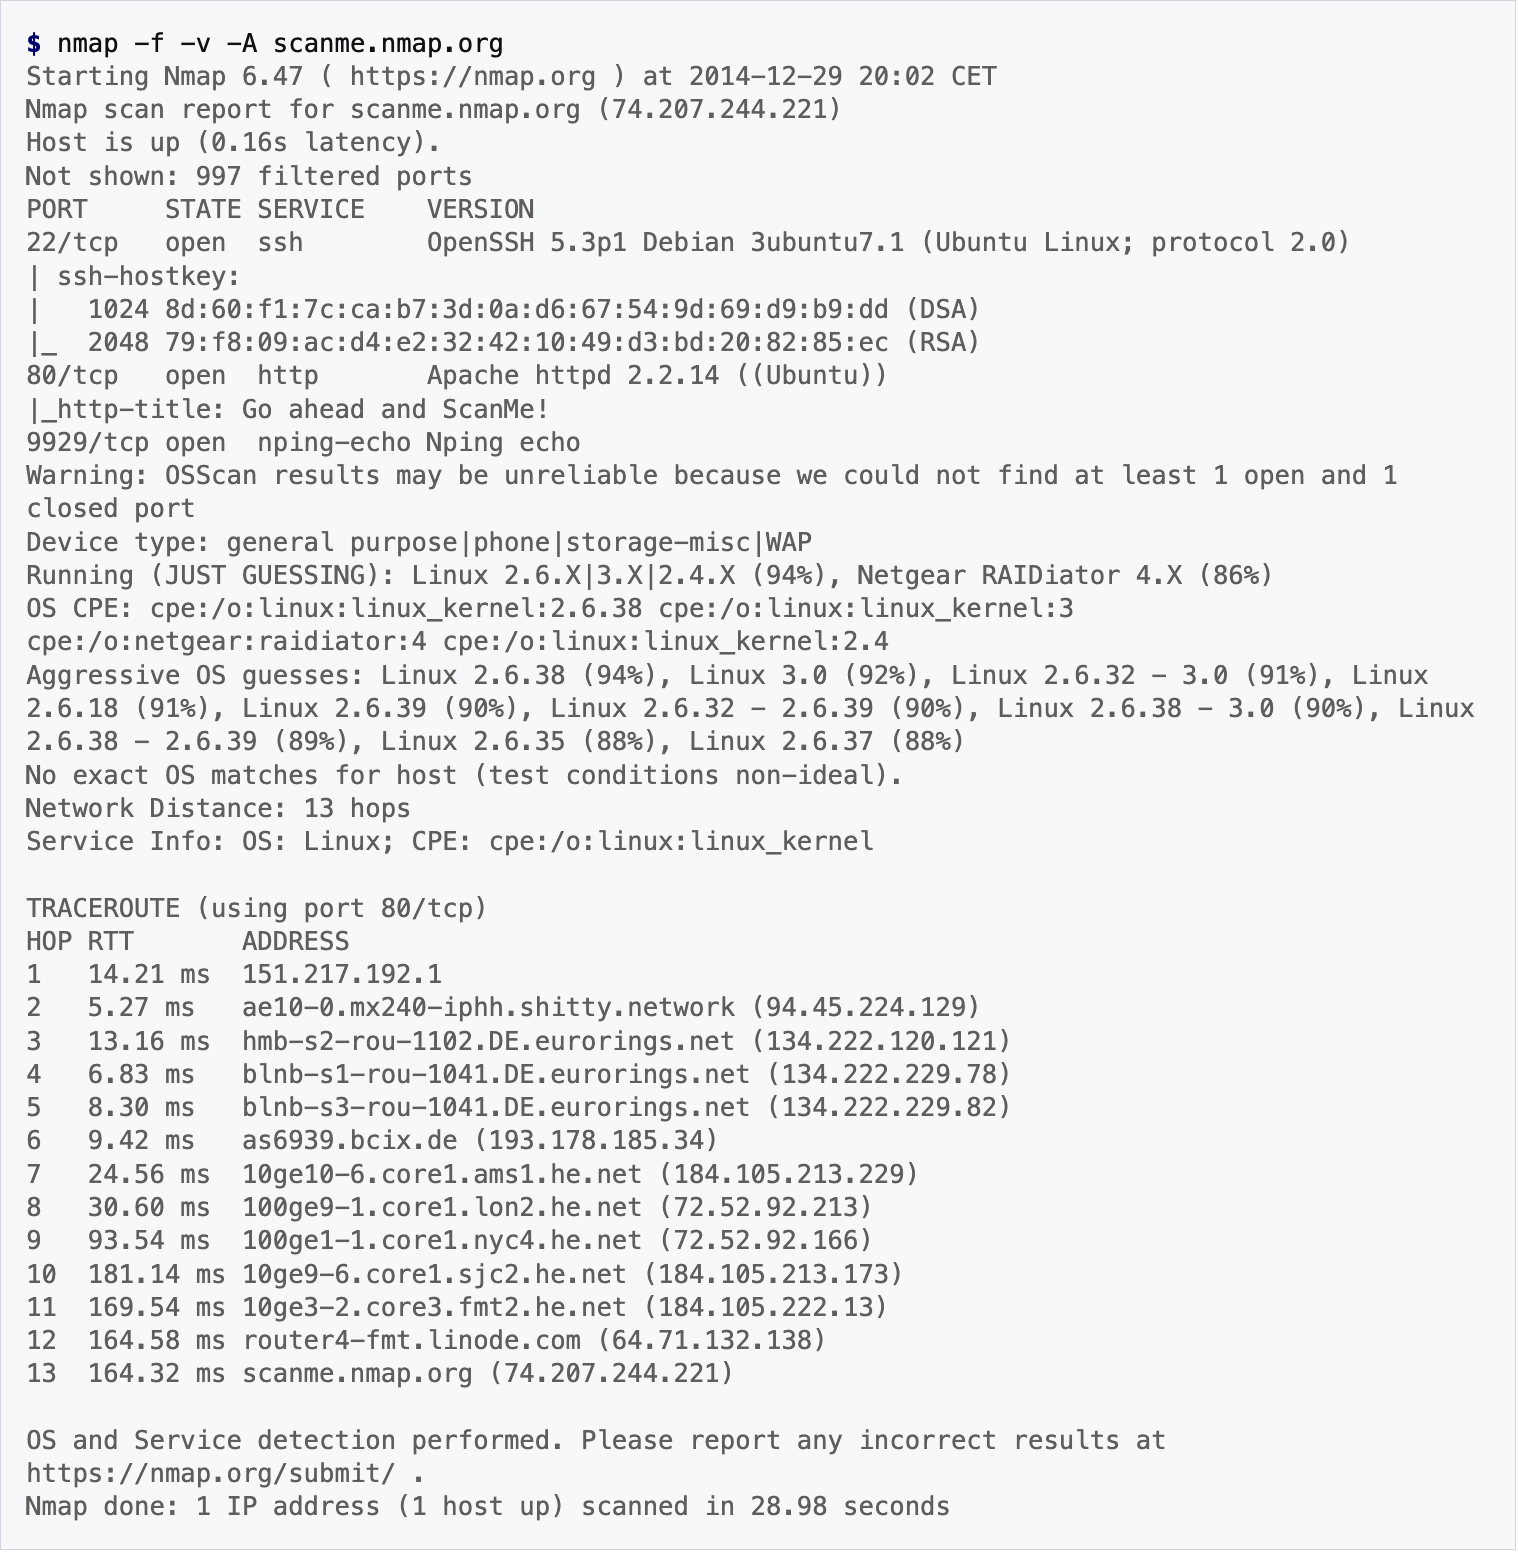
\includegraphics[width=0.7\textwidth]{images/NMAP_Wiki.png}
                \caption{Esempio di comando NMAP}
            \end{figure}
        \end{enumerate}
        \item \textbf{Vulnerabilty exploit:} Una volta completato l'ingresso nella rete aziendale, grazie alle prime due fasi citate, è ora possibile identificare e sfruttare al meglio altri buchi di sicurezza. Nella maggior parte dei casi, è necessario lasciare una via di accesso libera, comunemente detta \textit{"Backdoor"}, in modo da riuscire a bypassare i normali controlli di sicurezza e autenticazione e mantenere il login nell'infrastruttura. Una volta nella rete, ha inizio il vero monitoraggio dell'incident response che il Blue Team è capace di attuare; si inizia con il manomettere i sistemi ed ostacolare le funzioni offerte dall'azienda minacciata nonché la sottrarre informazioni sensibili dei clienti o dello stesso personale.
        \item \textbf{Physical security test:} Finora si è parlato di difese digitali, ma bisogna porre particolare attenzione anche alla sicurezza fisica dell'enterprise target.\\ 
        L'entrata ad aree sensibili è controllata da sistemi di autenticazione, convalidate spesso tramite chiavi di accesso magnetiche, passwords o addirittura biometriche. Il lavoro del Red Team può, quindi, includere misure quali il pedinamento o il furto in modo da entrare in possesso di lasciapassare e poter accedere a stanze altrimenti off-limits.\cite{red_team}\\
    \end{itemize}

    \noindent{\bfseries\Large Red Team vs Pentesting}\\[2em]
    Spesso il concetto di Red Teaming richiama l'idea simile, ma non equivalente, di Penetration Test; tuttavia vi sono delle differenze sostanziali che distinguono le due operazioni.\\
    Per definizione, il Penetration Test consiste in una serie di metodologie e tecniche con l'obiettivo di individuare il maggior numero di vulnerabilità in una rete; questo permette di mettere in evidenza quanto l'organizzazione sia a rischio e come gli attaccanti possano fare uso delle debolezze all'interno del sistema se non si applica al più presto una patch di sicurezza o un piano di gestione. Dalla suddetta descrizione, si evince la mancanza di un elemento fondamentale nella valutazione della protezione della propria infrastruttura in un'azienda cliente: l'abilità di riuscire a rilevare e prontamente reagire a uno specifico attacco informatico in corso. In base alla richiesta dunque, si può decidere se attuare un'operazione di Pentest o Red Teaming.\\[1em]
    \begin{minipage}[t]{0.5\textwidth}
        \centering
        \textbf{Red Teaming}
        \begin{itemize}
            \item Emula il comportamento di un avversario
            \item Usata per testare la resistenza di un enterprise a un attacco 
            \item Fornisce risultati utilizzabili nel rilevamento
        \end{itemize}
    \end{minipage}
    \begin{minipage}[t]{0.5\textwidth}
        \centering
        \textbf{Pentest}
        \begin{itemize}
            \item Ambito definito
            \item Identifica e sfrutta vulnerabilità
            \item Fornisce report sui ritrovamenti
            \item Più orientata alla prevenzione
        \end{itemize}
        \vspace{1.5em}
    \end{minipage}
    Le figure più influenti nel panorama della sicurezza informatica comprendono l'importanza dell'investimento nel settore di cybersecurity della propria azienda; è una spesa che nel lungo andare darà i suoi frutti, rafforzando le proprie difese ed evitando violazioni che rischiano di essere molto più costose di quanto si è investito.\\
    Un'operazione di Red Teaming è molto più completa, coinvolge molte più persone e risorse; inoltre, spesso e volentieri, può durare mesi interi; quindi, ci si può aspettare un costo maggiore. Difatti in media si stima una spesa dai 15.000€ in su; d'altro canto, un Penetration Test con un ambito ben definito costa dai 10.000€ in su.
    
    \subsection{Blue Team\label{blue}}
    Un Blue Team siede dalla parte opposta dell'esercizio di cybersecurity; si tratta di una squadra, spesso composta dal team di sicurezza dell'organizzazione, che utilizza gli strumenti e i servizi messi a disposizione da quest'ultima per rispondere ad un attacco imminente da parte del Red Team, ergo, sono specialisti in manovre di difesa. Spesso capita che l'enterprise non mandi nessun promemoria sull'inizio di una valutazione dei sistemi da parte del Red Team, facendo credere al Blue Team di essere bersaglio di una reale minaccia.\\
    Gli obiettivi principali di questa squadra risiedono principalmente nell'analisi e rivelazione di potenziali incidenti tramite la loro impronta digitale o nella risk intelligence; quando l'enterprise non è sotto attacco, si occupa di effettuare controlli regolari delle varie sotto-infrastrutture e, infine, come già detto, della preparazione del personale ad eventuali pericoli; questa attività è fondamentale e ad occuparsi di essa è proprio il Blue Team con dei briefing specializzati o corsi di apprendistato.\cite{blue_team}\\[1.5em]
    {\bfseries\Large{Competenze e Tools}}\\[2em]
    Le abilità dei singoli membri del team si concentrano sulla prevenzione, identificazione e risposta ai più recenti threat esistenti. Ma vi sono dei concetti chiave che ogni squadra deve evidenziare e mettere sul tavolo durante un incarico:
    \begin{itemize}
        \item \textbf{Network security:} Assicurare una forte sicurezza nell'infrastruttura di rete è, forse, l'incarico più cruciale e richiede profonde conoscenze in protocolli di rete, firewalls e VPNs.
        \item \textbf{Security tool proficiency:} Essere in grado di installare in ogni endpoint della rete dei sistemi di sicurezza essenziali, in grado riconoscere una minaccia dalla sua impronta digitale. Di seguito una lista degli strumenti essenziali:
        \begin{enumerate}
            \item \textbf{IDS:} Un Intrusion Detection System è un software o hardware capace di scovare la presenza di un intruso nel sistema o in un host grazie a tre componenti principali: sensori impiegati nella raccolta di pacchetti di dati o logs, analizzatori in grado di rilevare un agente esterno nel sistema ed un'interfaccia utente da cui è possibile configurare lo strumento. È possibile piazzare l'IDS in diversi punti strategici dell'infrastruttura di rete ed una sua dettagliata progettazione permette di identificare ed espellere un eventuale intruso prima che questi provochi danni alla rete.\\
            La scoperta di un estraneo è concettualmente legata alla supposizione che questo avrà un comportamento diverso da quello di un utente legittimo del network e alla rilevazione dell'impronta digitale che lasciano determinati pacchetti pericolosi.
            \item \textbf{IPS:} Un Intrusion Prevention System è un'estensione dell'IDS sopra citato. Essa include la capacità di effettuare un tentativo di blocco o prevenzione di un'attività illecita individuata. I metodi di rilevamento sono analoghi a quelli dell'Intrusion Detection System; una volta scoperto, è possibile fermare l'aggressore mediante diversi metodi: blocco o rimozione del flusso di contenuto dannoso, attivazione di altri dispositivi di sicurezza ed applicazione della security policy dell'organizzazione.
            \item \textbf{SIEM:} Acronimo per Security Information \& Event Management, permette ai team di sicurezza aziendali di eseguire una serie di funzioni di aggregazione, consolidamento ed ordinamento dei dati al fine di individuare minacce ed aderire ai requisiti di conformità delle informazioni.\\
            Alcune tra le funzionalità principali di questi sistemi sono: la gestione dei logs, la correlazione ed analisi degli eventi, monitoraggio ed avvertimenti di sicurezza e gestione delle conformità. 
        \end{enumerate}
        \item \textbf{Incident response:} Durante lo svolgimento di un attacco informatico, il membro della squadra deve saper riconoscere la strategia dell'attaccante ed i suoi TTPs. Questa abilità richiede la raccolta di informazioni da parte dei dispositivi precedentemente installati, i quali forniscono logs sui footprints delle tecniche in uso.
        \item \textbf{Threat Intelligence:} Un membro di un Blue Team deve essere in grado di individuare vulnerabilità e possibili punti di inizio di un vettore d'attacco nella rete, suggerire all'utente un eventuale rimedio a questo problema o agire autonomamente e neutralizzare il rischio.
    \end{itemize}

    \subsection{Cyber Range}
    Come spiegato al principio, gli attacchi cyber stanno avendo statisticamente la meglio sulle operazioni di risposta da parte dei team delle aziende. Questa è una situazione nata dalle poche risorse economiche investite e l'insufficiente preparazione degli impiegati, spesso dovuta a una mancata valutazione del rischio. Tale informazione viene spesso realizzata solo dopo che i sistemi sono già stati compromessi. Il concetto si estende agli utenti individuali essendo anch'essi potenziali bersagli, soprattutto se occupano una posizione di rilievo nell'azienda.
    I cyber range vengono in soccorso di questa lacuna, essendo degli ambienti virtuali per la formazione, la verifica e la ricerca sulla cybersecurity. Essi simulano reti e attacchi informatici reali. Consentono di addestrare il proprio personale nonché analizzare problematiche abbastanza complesse all'interno di un environment sicuro ed isolato; è possibile configurare anche minacce specifiche e comuni quali ransomware o phising.\\
    Il National Institute of Standards and Technology (NIST) è un'azienda non regolamentare, fondata nel 1901, che promuove l'innovazione attraverso il progresso della scienza, degli standard e della tecnologia delle misurazioni ed il suo Cybersecurity Framework è spesso utilizzato nello sviluppo dei cyber range: si tratta di standard, linee guida e best practice per aiutare le organizzazioni a migliorare la loro gestione dei rischi per la sicurezza.\cite{ibm_cyberRange}\\[1.5em]
    {\bfseries\Large{Struttura tecnica}}\\[1em]
    I componenti tecnici che collaborano per creare un ambiente realistico e monitorato per le varie esercitazioni sono:
    \begin{description}
        \item[RLMS ${\rightarrow}$] Il Range Learning Management System combina le caratteristiche di un semplice sistema di gestione dell'apprendimento (LMS) con le esigenze richieste per lo sviluppo del cyber range. Si tratta del componente fulcro del monitoraggio dei progressi e della valutazione delle pratiche svolte.
    \end{description}
    \begin{figure}[H]
        \centering
        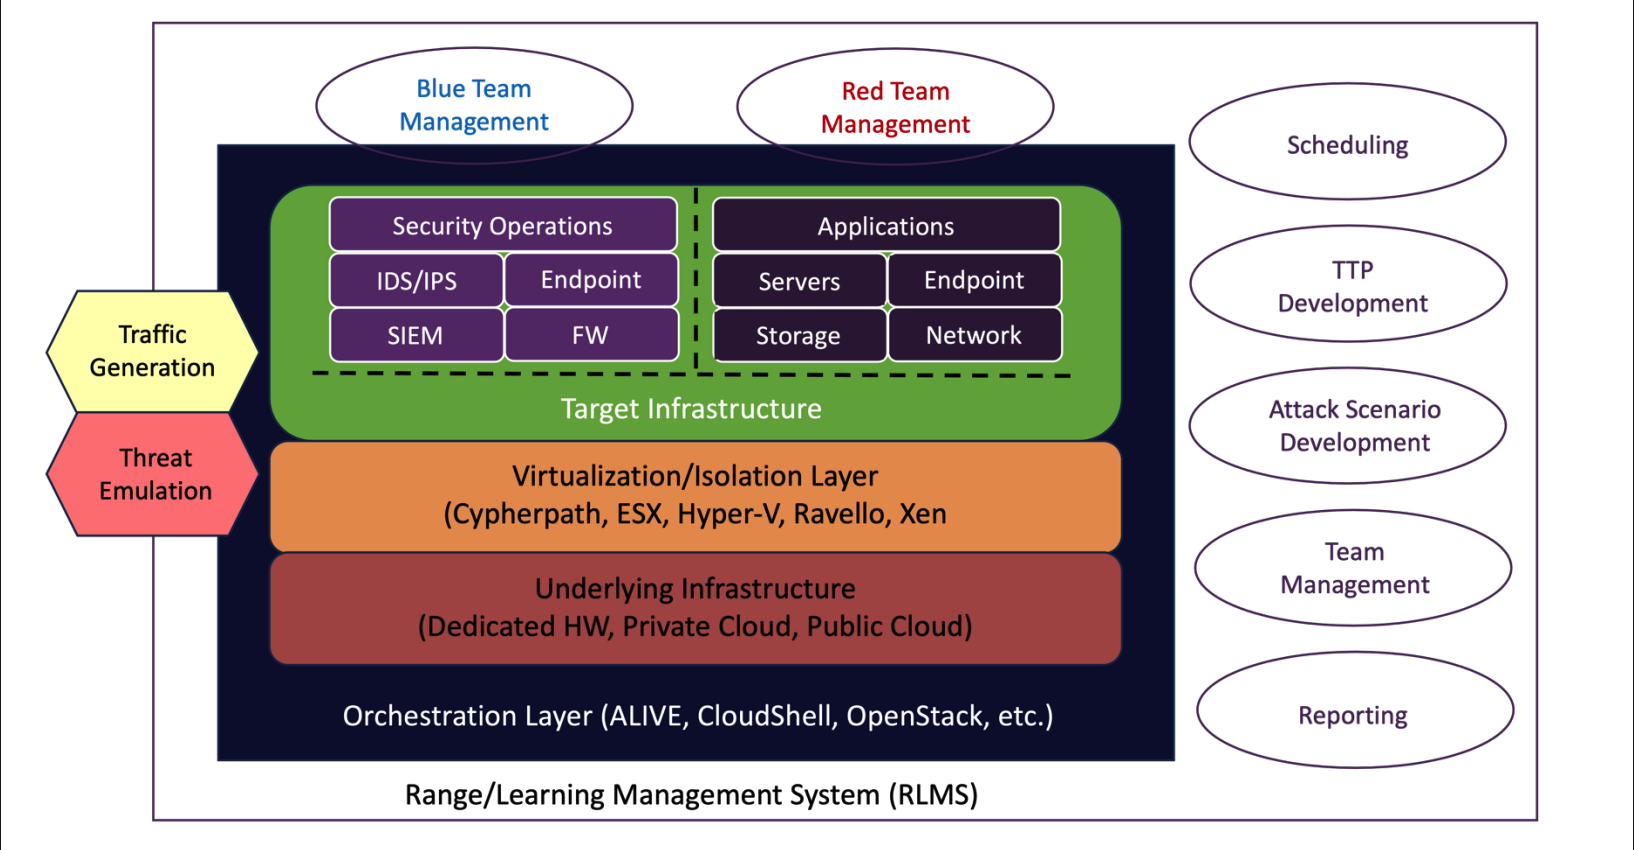
\includegraphics[width=0.85\linewidth, trim=2 0 2 0, clip]{images/RLMS.png}
        \caption{Diagramma di un RLMS}
    \end{figure}
    \begin{description}
        \item[Livello di orchestrazione $\rightarrow$] Alimentato dall'input proveniente dal RLMS, coordina i vari servizi all'interno del cyber range. Integra l'infrastruttura sottostante, la virtualizzazione e il target, supportando inoltre un'estensibilità dinamica del range attraverso la sua compatibilità con dei cloud privati o pubblici e con le infrastrutture cablate dedicate.
        \item[Infrastruttura sottostante $\rightarrow$] Include server, reti e storage, costituiti da un insieme di dispositivi fisici quali router o firewall, sebbene molti fornitori di ranges stiano migrando verso un'infrastruttura virtuale software-based.\\
        La scelta di quest'ultima impatta in modo cruciale sul realismo dell'esercitazione ed una considerazione importante ruota attorno al livello di supporto richiesto al fine di soddisfare le richieste del cliente.
        \item[Livello di virtualizzazione $\rightarrow$] Al fine di ridurre il numero di apparecchiature fisiche, molti adottano la virtualizzazione basata su due approcci comuni: hypervisor-based e infrastruttura definita su software. Il grado di disintermediazione tra l'infrastruttura sottostante e il target è fondamentale nella progettazione di un ambiente realistico e, grazie all'astrazione, è possibile creare una barriera tra queste due poiché possono contenere potenziali vettori di attacco.
        \item[Infrastruttura target $\rightarrow$] Si riferisce all'ambiente simulato vero e proprio in cui è possibile allenarsi; nei cyber range più avanzati, questi ambienti possono includere profili di server commerciali disponibili, endpoints, firewalls, ecc...\\
        Durante l'esercitazione, il RLMS genera scripts capaci di guidare il livello di orchestrazione ad organizzare il target; difatti, contengono dettagli quali range di indirizzi IP, server stacks e simili. 
    \end{description}
    \vspace{0.5em}
    {\bfseries\Large{Tipologie}}\\[1em]
    I cyber range si sono evoluti in distinte tipologie, in modo da soddisfare ogni singolo use case o necessità di miglioramento nel settore di ogni azienda cliente. È bene prendere atto delle principali differenze oltre alle diverse funzionalità rese disponibili da ogni categoria diversa di range. Di seguito, una classificazione con annessa descrizione:
    \begin{itemize}
        \item \textbf{Simulation ranges:} Implica la creazione di un ambiente di rete sintetico atto a replicare il comportamento dei componenti reali. La simulazione avviene all'interno di istanze virtuali per i vantaggi esplicitati precedentemente.
        \item \textbf{Overlay ranges:} Utilizzano direttamente la rete e i sistemi dell'enterprise; aumentandone il grado di realismo, ma, al contempo, anche il costo, il numero di componenti e il rischio di compromettere l'infrastruttura sottostante.
        \item \textbf{Emulation ranges:} Consiste nell'implementazione del range in una rete dedicata e mappata direttamente sull'infrastruttura fisica dell'azienda.
        \item \textbf{Hybrid ranges:} Formata da una combinazione dei ranges citati in precedenza, creando, quindi, un ambiente che soddisfa richieste specifiche.
    \end{itemize}
    